% Résultats
\chapter{Résultats}
Les résultats de la migration sont présentés sous forme de documents JSON pour chaque entité, illustrant les avantages de la dénormalisation et les structures simplifiées obtenues. On peut visualiser les résultats en effectuant des requetes vers la base de données NoSQL et donc au JSON car le format JSON est utilisé dans redis et mongo en tant que document.

Pour illustrer les avantages de la dénormalisation, nous avons utilisé des exemples de requêtes et de jointures pour montrer comment les données peuvent être manipulées et agrégées de manière plus efficace. Ces exemples sont présentés dans la section suivante.

\section{Exemple de requêtes et de jointures}

En ayant convertit nos tables SQL en JSON, nous pouvons normaliser les requêtes et les jointures pour manipuler les données de manière plus efficace que les données viennent d'un fichier JSON, récupéré par redis ou par mongo.

\section{Comparaison des Performances}

La figure~\ref{fig:image1} montre les performances des requêtes avec les données d'origine, tandis que la figure~\ref{fig:image2} montre les performances avec un grand volume de données.

On peut voir que pour un nombre de données faibles, le temps de requêtes avec Redis en important en JSON est plus faible que avec MongoDB en JSON et avec des recherches MongoDB (Pipelines). Cependant, avec un volume de données plus important, les performances sont plus élevées avec MongoDB (Pipelines) et en stocker les données Mongo en JSON.\@

\begin{figure}[H]
  \centering
  \begin{subfigure}[t]{0.45\textwidth}
    \centering
    \includegraphics[width=\linewidth]{small/execution_times_comparison_total.png}
    \caption{Comparaison des performances avec les données d'origine}
    \label{fig:image1}
  \end{subfigure}
  \hfill
  \begin{subfigure}[t]{0.45\textwidth}
    \centering
    \includegraphics[width=\linewidth]{execution_times_comparison_total.png}
    \caption{Comparaison des performances avec un grand volume de données}
    \label{fig:image2}
  \end{subfigure}
  % Optionnel : Ajouter une légende globale pour l'ensemble des images
  \caption{Comparaison des performances avec les données d'origine et avec un grand volume de données}
  \label{fig:comparaison_performances}
\end{figure}
